\section{Resultados Obtidos}

\subsection{Comparação de leitura e escrita de arquivo no Pandas}

Neste ponto, verificamos o tempo de execução na leitura e gravação de arquivos, utilizando arquivo compactado em CSV e outro em Parquet. Dado que o arquivo foi carregado em Python, prosseguimos com os testes. Quanto menor o tempo, melhor. Vemos que o Parquet vence nos cenários de Leitura e Gravação. Perde apenas no tamanho do arquivo compactado. Vide a Tabela \ref{tab1}. Os códigos do Pandas utilizados são: \textit{to\_csv, read\_csv, to\_parquet, read\_parquet}, e podem ser encontrados na documentação do mesmo \cite{PandasDocumentation}.

\begin{table}[htbp]
	\caption{Comparação CSV vs Parquet}
	\begin{center}
		\begin{tabular}{|c|c|c|c|c|}
			\hline
			\textbf{Arquivo} & \textbf{Gravação} & \textbf{Leitura} & \textbf{Tamanho} \\
			\hline
			CSV              & 106s                & 29s              & 305 mb           \\
			\hline
			Parquet          & 70s                 & 12s              & 329 mb           \\
			\hline
		\end{tabular}
		\label{tab1}
	\end{center}
\end{table}

Desta forma, os resultados preliminares mostram que o tempo de processamento deste dataset no formato Parquet foi 34\% mais rápido do que no formato CSV. Além disso, o Parquet foi XX\% mais rápido na leitura do que o CSV. Um ganho significativo, se considerado os custos de processamento e de volume de dados utilizados na Ciência de Dados.

Com relação ao tamanho, apesar do resultado ter sido pior, é importante lembrar de um outro estudo em que a empresa Databricks realizou um comparativo de performance e economia de espaço. Foi possível verificar uma economia com recursos de armazenamento de 87\% \cite{Databricks}. Isso indica que é possível que os ganhos no armazenamento neste formato cresçam de acordo com o aumento do tamanho dos datasets.
	
\subsection{Análise otimizada de grande volume de dados utilizando amostra estratificada}
	
Neste ponto há dois fatores a serem analisados, uma é a vantagem de uma amostra estratificada e a outra é a comparação de uma visualização no formato de grafo em contraste a um de tabela. 
	
\paragraph{Amostra Estratificada} Utilizando os arquivos gerados \hyperref[arq:1A]{Arquivo 1-A}, \hyperref[arq:1B]{Arquivo 1-B}, \hyperref[arq:1C]{Arquivo 1-C}, \hyperref[arq:1D]{Arquivo 1-D}, demos a carga no Neo4J.
	
Na Figura \ref{fig1} abaixo, temos dois arquivos não estratificados. O da esquerda com 1.000 registros e o da direita com 10.000 registros.
	
\begin{figure}[htbp]
	\centerline{
		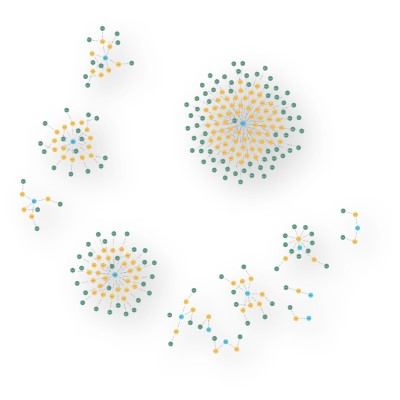
\includegraphics[width=40mm,scale=0.4]{assets/Imagem1.jpg}
	}
	\caption{Amostras Não Estratificadas dos \hyperref[arq:1A]{Arquivo 1-A} e \hyperref[arq:1B]{Arquivo 1-B}}
	\label{fig1}
\end{figure}
